\documentclass[t,12pt,numbers,fleqn,usenames,xcolor=dvipsnames]{beamer}
%\documentclass[t,12pt,numbers,fleqn,handout]{beamer}

\usepackage{amsmath}
\usepackage{mathtools}
\usepackage{amsfonts}
\usepackage{paralist}
\usepackage{latexsym}
\usepackage{amssymb}
\usepackage{stmaryrd}
\usepackage{phonetic}
\usepackage{wasysym}
\usepackage{pgf}
\usepackage{tikz}
\usepackage{url}
\usetikzlibrary{arrows}
\usepackage{array}
\usepackage{pgfpages} 
\usepackage{multirow} 
\usepackage{graphicx}
\usepackage{color}
\usepackage{listings,lstautogobble}
\lstset{
	basicstyle=\ttfamily,
	mathescape
}
\usepackage{calc}
\usepackage{tikz}
\usepackage{tikz-cd}
\usetikzlibrary{tikzmark,calc,decorations.pathreplacing,positioning,fadings}
\usepackage{hyperref}
\usepackage{verbatim}
\usepackage{fancyvrb}
\usepackage{tabularx}
\usepackage{tikz}
\usepackage{tikz-cd}
\usetikzlibrary{cd}
\usepackage{graphicx}
\usepackage{collectbox}
\usepackage{tabularx}
\usepackage{wrapfig}
\usepackage{lscape}
\usepackage{textcomp}
\usepackage[show]{ed}
\usepackage{adjustbox}
\setlength{\arrayrulewidth}{1mm}
\setlength{\tabcolsep}{18pt}
\renewcommand{\arraystretch}{1.5}
\hypersetup{colorlinks=true,
    linkcolor=blue,
    citecolor=blue,
    filecolor=blue,
    urlcolor=blue,
    unicode=false}

\usepackage{macros/myMacros}
\usepackage{macros/local}
\usepackage{macros/basics}

%\usepackage[backend=biber,style=numeric, sorting = none,
%maxbibnames=99, defernumbers=true, isbn = true]{biblatex}
%\addbibresource{refs.bib}

% To include lagda 
%\usepackage{latex/agda}
%\usepackage{ucs}
%\usepackage[utf8x]{inputenc}
%\usepackage{autofe}
%\usepackage{fancyvrb}
%\DefineVerbatimEnvironment
%{code}{Verbatim}


\lstset{language=lisp,basicstyle=\ttfamily,breaklines=true,showspaces=false,showstringspaces=false,breakatwhitespace=true,texcl=true,escapeinside={\%*}{*)}}
\tikzstyle{stuff_fill}=[rectangle,draw,fill=black!20,minimum size=1.4em]


\usepackage{fancybox}

\mode<presentation>{}


\usetheme{default}
\setbeamertemplate{navigation symbols}{} 
\setbeamertemplate{itemize item}[ball]
\setbeamersize{text margin left = 4mm}
\setbeamersize{text margin right = 4mm}

%\input{def-beamer}

\title{Diagram Combinators in MMT}
\subtitle{Approach to Building Large Libraries}
\author{Florian Rabe$^1$ and \underline{Yasmine Sharoda$^2$}}
\institute{$^1$FAU Erlangen-N{\"u}rnberg, Germany and LRI, Universit{\'e} Paris Sud, France  \and
	$^2$ McMaster University, Canada}
\date{}
	
\newcommand\textline[4][t]{%
	\par\smallskip\noindent\parbox[#1]{.333\textwidth}{\raggedright\texttt{+}#2}%
	\parbox[#1]{.333\textwidth}{\centering#3}%
	\parbox[#1]{.333\textwidth}{\raggedleft\texttt{#4}}\par\smallskip%
}	

\setbeamertemplate{footline}[frame number]

\newcommand{\icsg}{\cn{IdempotentCommutativeSemigroup}\xspace}
	
\begin{document}

\begin{frame}
\titlepage
\end{frame}


\section{Motivation}

\begin{frame}[fragile]{Motivation}
\begin{itemize}
\item Formal libraries are growing 
\pause 
\item Theory graph structure 
\begin{itemize}
	\item A network of little theories 
\end{itemize}
\item Theory Combinators 
\end{itemize}
\end{frame}

\begin{frame}[fragile]{Motivation}
\begin{itemize}
	\item Theories are becoming hard to manage
\end{itemize}
\pause 
\vspace{0.5cm}
Example: 
\scriptsize{
	\begin{center}
		\begin{tikzpicture}[scale=.8]
		\node (M)    at (0,0)      {\Magma(U,*)};
		\node (CM) at (-4,-1) {\CommMagma};
		\node (SG)  at (0,-1)   {\Semigroup};
		\node (IM)  at  (4,-1)   {\IdempMagma};
		\draw[mono](M) -- (CM);
		\draw[mono](M) -- (SG); 
		\draw[mono](M) -- (IM);
		\node (CSG)  at (-5,-2)   {\CommutativeSemigroup};
		\node (ISG)    at (5,-2)    {\IdempotentSemigroup};
		\node (ICM)    at (0,-2)    {\IdempotentCommutativeMagma};
		\node (ACSG)  at (0,-3)   {\IdempotentCommutativeSemigroup (U,*,assoc,idemp,comm)};
		\draw[mono](CM) -- (CSG);
		\draw[mono](CM) -- (ICM);
		\draw[mono](IM) -- (ISG); 
		\draw[mono](IM) -- (ICM);
		\draw[mono](SG) -- (ISG); 
		\draw[mono](SG) -- (CSG);
		\draw[mono](CSG) -- (ACSG);
		\draw[mono](ISG) -- (ACSG);
		\draw[mono](ICM) -- (ACSG);
		\end{tikzpicture}
\end{center}}
\pause
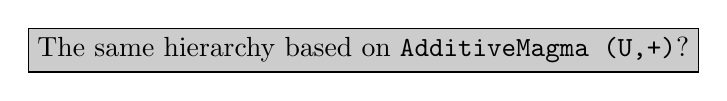
\begin{tikzpicture}
\draw (1,1) node [stuff_fill] {The same hierarchy based on \verb|AdditiveMagma (U,+)|?};
\end{tikzpicture}
\end{frame}

\begin{frame}
\frametitle{Motivation}
\begin{itemize}
	\item Structure library into network of diagrams 
	\item Diagram operators for computing entire diagrams 
\end{itemize}
\end{frame}

\begin{comment}[fragile]{Motivation}
Building the algebraic hierarchy as a theory graph 
\begin{itemize}
	\item[] From: \textcolor{Blue}{\Magma \cn{(U,\_*\_)}}
	\item[] To: \textcolor{Blue}{\icsg \\ \qquad  \cn{(U,\_*\_,assoc,comm,idemp)}} 
\end{itemize}
\pause

\begin{onlyenv}<1>
Extremely Modular -- Tiny Theories 
\begin{itemize}
	\item Adding one definition at a time 
	\item All intermediate theories are defined 
\end{itemize}
\end{onlyenv}

\begin{onlyenv}<2>
	\scriptsize{
		\begin{center}
			\begin{tikzpicture}[scale=.8]
			\node (M)    at (0,0)      {\Magma};
			\node (CM) at (-4,-1) {\CommMagma};
			\node (SG)  at (0,-1)   {\Semigroup};
			\node (IM)  at  (4,-1)   {\IdempMagma};
			\draw[mono](M) -- (CM);
			\draw[mono](M) -- (SG); 
			\draw[mono](M) -- (IM);
			\node (CSG)  at (-5,-2)   {\CommutativeSemigroup};
			\node (ISG)    at (5,-2)    {\IdempotentSemigroup};
			\node (ICM)    at (0,-2)    {\IdempotentCommutativeMagma};
			\node (ACSG)  at (0,-3)   {\IdempotentCommutativeSemigroup};
			\draw[mono](CM) -- (CSG);
			\draw[mono](CM) -- (ICM);
			\draw[mono](IM) -- (ISG); 
			\draw[mono](IM) -- (ICM);
			\draw[mono](SG) -- (ISG); 
			\draw[mono](SG) -- (CSG);
			\draw[mono](CSG) -- (ACSG);
			\draw[mono](ISG) -- (ACSG);
			\draw[mono](ICM) -- (ACSG);
			\end{tikzpicture}
	\end{center}}
\end{onlyenv}
\end{comment}

\begin{comment}[fragile]{Motivation}
\begin{enumerate}
	\item[1.] Flat Theories 
	\scriptsize{
		\begin{lstlisting}
Theory $\icsg$ := {
  U : type 
  $\_\circ\_$ : U $\rightarrow$ U $\rightarrow$ U 
  associativity : $\cdots$
  commutativity : $\cdots$
  idempotence : $\cdots$
}
		\end{lstlisting}}
	\scriptsize{
		\begin{center}
			\begin{tikzpicture}[scale=.8]
			\node (M)    at (0,0)      {\Magma};
			\node (CM) at (-4,-1) {\CommMagma};
			\node (SG)  at (0,-1)   {\Semigroup};
			\node (IM)  at  (4,-1)   {\IdempMagma};
			\node (CSG)  at (-5,-2)   {\CommutativeSemigroup};
			\node (ISG)    at (5,-2)    {\IdempotentSemigroup};
			\node (ICM)    at (0,-2)    {\IdempotentCommutativeMagma};
			\node (ACSG)  at (0,-3)   {\icsg};
			\end{tikzpicture}
	\end{center}}
\end{enumerate}
\end{comment}

\begin{comment}[fragile]{Motivation}
\begin{enumerate}
	\item[1.] Flat Theories 
	\item[2.] Theory Formation Operators 
	\begin{itemize}
		\item Extension / Inclusions 
\scriptsize{
	\begin{lstlisting}
Theory CommutativeMagma{ 
  includes Magma 
  commutativity : $\cdots$  
}	
$\cdots$
Theory CommutativeSemigroup{ 
  includes CommutaitveMagma 
  includes Semigroup 
}	
\end{lstlisting}}		
	\end{itemize}
\end{enumerate}
\scriptsize{
	\begin{center}
		\begin{tikzpicture}[scale=.8]
		\node (M)    at (0,0)      {\Magma};
		\node (CM) at (-4,-1) {\CommMagma};
		\node (SG)  at (0,-1)   {\Semigroup};
		\node (IM)  at  (4,-1)   {\IdempMagma};
		\node (IM)  at  (4,-1)   {\IdempMagma};
		\node (CSG)  at (-5,-2)   {\CommutativeSemigroup};
		\node (ISG)    at (5,-2)    {\IdempotentSemigroup};
		\node (ICM)    at (0,-2)    {\IdempotentCommutativeMagma};
		\node (ACSG)  at (0,-3)   {\icsg};		
		\draw[mono](M) -- (CM);
		\draw[mono](M) -- (SG); 
		\draw[mono](M) -- (IM);
		\end{tikzpicture}
\end{center}}
\end{comment}

\begin{comment}[fragile]{Motivation}
\begin{enumerate}
	\item[1.] Flat Theories 
	\item[2.] Theory Formation Operators 
	\begin{itemize}
		\item Extension / Inclusions 
		\item Colimit
	\end{itemize}
\end{enumerate}
\scriptsize{
	\begin{lstlisting}
	IdempotentMagma := Magma extended_by {idemp : }
	CommutativeMagma := Magma extended_by {comm : }
	Semigroup := Magma extended_by {assoc : }
	\end{lstlisting}}
\scriptsize{
	\begin{center}
		\begin{tikzpicture}[scale=.8]
		\node (M)    at (0,0)      {\Magma};
		\node (CM) at (-4,-1) {\CommMagma};
		\node (SG)  at (0,-1)   {\Semigroup};
		\node (IM)  at  (4,-1)   {\IdempMagma};
		\draw[mono](M) -- (CM);
		\draw[mono](M) -- (SG); 
		\draw[mono](M) -- (IM);
		\end{tikzpicture}
\end{center}}
\end{comment}

\begin{comment}[fragile]{Motivation}
\begin{enumerate}
	\item[1.] Flat Theories 
	\item[2.] Theory Formation Operators 
\end{enumerate}	
	\scriptsize{
	\begin{lstlisting}
IdempotentMagma := Magma extended_by {idemp : }
CommutativeMagma := Magma extended_by {comm : }
Semigroup := Magma extended_by {assoc : }
IdempotentSemigroup := Combine IdempotentMagma Semigroup
CommutativeSemigroup := Combine CommutativeMagma Semigroup 
IdempotentCommutative := 
     Combine IdempotentMagma CommutativeMagma 
IdempotentCommutativeSemigroup := 
     Combine IdempotentMagma CommutativeMagma Semigroup
	\end{lstlisting}}
\scriptsize{
	\begin{center}
		\begin{tikzpicture}[scale=.8]
		\node (M)    at (0,0)      {\Magma};
		\node (CM) at (-4,-1) {\CommMagma};
		\node (SG)  at (0,-1)   {\Semigroup};
		\node (IM)  at  (4,-1)   {\IdempMagma};
		\draw[mono](M) -- (CM);
		\draw[mono](M) -- (SG); 
		\draw[mono](M) -- (IM);
		\node (CSG)  at (-5,-2)   {\CommutativeSemigroup};
		\node (ISG)    at (5,-2)    {\IdempotentSemigroup};
		\node (ICM)    at (0,-2)    {\IdempotentCommutativeMagma};
		\node (ACSG)  at (0,-3)   {\IdempotentCommutativeSemigroup};
		\draw[mono](CM) -- (CSG);
		\draw[mono](CM) -- (ICM);
		\draw[mono](IM) -- (ISG); 
		\draw[mono](IM) -- (ICM);
		\draw[mono](SG) -- (ISG); 
		\draw[mono](SG) -- (CSG);
		\draw[mono](CSG) -- (ACSG);
		\draw[mono](ISG) -- (ACSG);
		\draw[mono](ICM) -- (ACSG);
		\end{tikzpicture}
\end{center}}
\pause
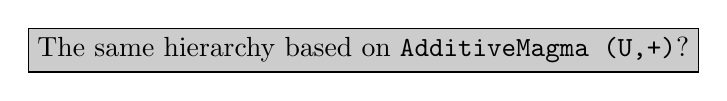
\begin{tikzpicture}
\draw (1,1) node [stuff_fill] {The same hierarchy based on \verb|AdditiveMagma (U,+)|?};
\end{tikzpicture}
\end{comment}

\begin{comment}[fragile]{Motivation}
\begin{enumerate}
	\item[1.] Flat Theories 
	\item[2.] Theory Formation Operators 
\end{enumerate}	
\scriptsize{
	\begin{lstlisting}
	IdempotentMagma := Magma extended_by {idemp : }
	CommutativeMagma := Magma extended_by {comm : }
	Semigroup := Magma extended_by {assoc : }
	IdempotentSemigroup := Combine IdempotentMagma Semigroup
	CommutativeSemigroup := Combine CommutativeMagma Semigroup 
	IdempotentCommutative := 
	Combine IdempotentMagma CommutativeMagma 
	IdempotentCommutativeSemigroup := 
	Combine IdempotentMagma CommutativeMagma Semigroup
	\end{lstlisting}}
\scriptsize{
	\begin{center}
		\begin{tikzpicture}[scale=.8]
		\node (M)    at (0,0)      {\Magma};
		\node (AM) at (1,0)    {$\cn{AdditiveMagma}$}
		\node (CM) at (-4,-1) {\CommMagma};
		\node (SG)  at (0,-1)   {\Semigroup};
		\node (IM)  at  (4,-1)   {\IdempMagma};
		\draw[mono](M) -- (CM);
	%	\draw[arrow] (M) -- (AM)
		\draw[mono](M) -- (SG); 
		\draw[mono](M) -- (IM);
		\node (CSG)  at (-5,-2)   {\CommutativeSemigroup};
		\node (ISG)    at (5,-2)    {\IdempotentSemigroup};
		\node (ICM)    at (0,-2)    {\IdempotentCommutativeMagma};
		\node (ACSG)  at (0,-3)   {\IdempotentCommutativeSemigroup};
		\draw[mono](CM) -- (CSG);
		\draw[mono](CM) -- (ICM);
		\draw[mono](IM) -- (ISG); 
		\draw[mono](IM) -- (ICM);
		\draw[mono](SG) -- (ISG); 
		\draw[mono](SG) -- (CSG);
		\draw[mono](CSG) -- (ACSG);
		\draw[mono](ISG) -- (ACSG);
		\draw[mono](ICM) -- (ACSG);
		\end{tikzpicture}
\end{center}}
\pause
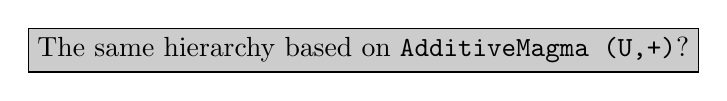
\begin{tikzpicture}
\draw (1,1) node [stuff_fill] {The same hierarchy based on \verb|AdditiveMagma (U,+)|?};
\end{tikzpicture}
\end{comment}

\begin{comment}[fragile]{Motivation}
\begin{enumerate}
	\item[1.] Flat Theories 
	\item[2.] Theory Formation Operators
	\item[3.] \textcolor{Blue}{Diagram Formation Operators}
\end{enumerate}
\end{comment}

\begin{frame}[fragile]{Diagram Definition}
A \textbf{diagram} $D$ consists of
\begin{itemize}
	\item a list of \textbf{nodes}: \node{l}{D_n(l)} 
	\pause
	\item a list of \textbf{edges}, \edge{l}{d}{c}{D_E(l)} 
	\pause
	\item an optional label $\dist{D}$ of a node --- the \textbf{distinguished} node
	\item an optional label $\iedge{l}{d}{c}{D(l)}$ of an arrow -- the \textbf{implicit} arrow 
\end{itemize}
\end{frame}



\begin{frame}[fragile]{Diagram Operations}
Based on 
\begin{itemize}
	\item Theory Formation Operations
	\item Set-Theoretic Operations 
	\item Batch Formation of Theories 
\end{itemize}
\pause 
Running Example: Building the algebraic hierarchy as a theory graph 
\begin{itemize}
	\item[] From: \textcolor{Blue}{\Magma \cn{(U,\_*\_)}}
	\item[] To: \textcolor{Blue}{\icsg \\ \qquad  \cn{(U,\_*\_,assoc,comm,idemp)}} 
\end{itemize}
\end{frame}

\begin{frame}[fragile]{Diagram Operations}
Based on 
\begin{itemize}
	\item \textcolor{Blue}{Theory Formation Operations}
	\item Set-Theoretic Operations 
	\item Batch Formation of Theories 
\end{itemize}
\end{frame}
\begin{comment}[fragile]{Diagram: Examples}
\scriptsize{
	\begin{lstlisting}
diagram Semigroup := Magma extended_by {associativity : $\cdots$}
diagram CommutativeMagma := Magma extended_by {commutativity : $\cdots$}
	\end{lstlisting}}
\begin{center}
\begin{tikzcd}
	Magma \arrow[r,blue] & \textcolor{blue}{\cn{Semigroup}} \\ 
	Magma \arrow[r,blue] & \textcolor{blue}{\cn{CommutativeMagma}}	
\end{tikzcd} 
\end{center}
\scriptsize{
	\begin{lstlisting}
diagram PointedMagma := Combine Semigroup CommutativeMagma
	\end{lstlisting}}
\begin{tikzcd}
	Magma \arrow[r] \arrow[d] \arrow[rd,blue]
	& Semigroup \arrow[d]  \\
	CommutativeMagma \arrow[r] & \textcolor{blue}{\cn{CommutativeSemigroup}}
\end{tikzcd} 
\end{comment}


\begin{frame}[fragile]{Theory Formation Operations}
Interpreting combinators from MathScheme \cite{mathscheme_theoexp} as diagram operations 
\end{frame}

\begin{frame}[fragile]{Theory Formation Operations}
\begin{enumerate}
\item[1.] Extension
\footnotesize 
\begin{lstlisting}
diagram d$^{\prime}$ := d extended_by $\Sigma$ 
\end{lstlisting}
\pause
\begin{columns}
	\begin{column}{0.45\textwidth}
\begin{block}{\footnotesize{Input Diagram}}
\begin{tikzcd}
	\arrow[r] & \dist{D}  
\end{tikzcd} 
\end{block}	
	\end{column}
	\begin{column}{ 0.45\textwidth}		
\begin{block}{\footnotesize{Output Diagram}}
\begin{tikzcd}
	\arrow[r] & \dist{D} \arrow[r,,blue] & \textcolor{blue}{\pres} \\%\dist{D} \rtimes \Sigma}  \\
\end{tikzcd} 
\end{block}			
\end{column}
\end{columns}
\end{enumerate}
\pause
\footnotesize
\begin{lstlisting}
diagram Magma = Carrier  extended$\_$by {_*_:U $\to$ U $\to$ U}
diagram Semigroup = Magma extended$\_$by {assoc : $\cdots$}
\end{lstlisting}
\begin{tikzcd}
\dist{Carrier} \arrow[r,hook] & \dist{Magma} \arrow[r,hook,blue] & \textcolor{blue}{\pres}
\end{tikzcd}
\end{frame}

\begin{frame}[fragile]{Theory Formation Operations}
\begin{enumerate}	
	\item[2.] Rename 
\footnotesize			
	\begin{lstlisting}
diagram d$^{\prime}$ := d rename r 
	\end{lstlisting}
\begin{columns}
	\small
	\begin{column}{0.45\textwidth}
		\begin{block}{\footnotesize Input Diagram}
			\begin{tikzcd}
				\arrow[r] & \dist{D}  
			\end{tikzcd} 
		\end{block}	
	\end{column}
	\begin{column}{ 0.45\textwidth}
		\begin{block}{\footnotesize Output Diagram}
			\begin{tikzcd}
				\arrow[r] & \dist{D} \arrow[r,,blue] & \textcolor{blue}{\pres} \\%\dist{D} \rtimes \Sigma}  \\
			\end{tikzcd} 
		\end{block}			
	\end{column}
\end{columns}
\end{enumerate}
\footnotesize
\begin{lstlisting}
diagram AdditiveMagma = Magma rename { * $\rewrites$ +}
\end{lstlisting}
\begin{tikzcd}
	\dist{Carrier} \arrow[r,hook] & \dist{Magma} \arrow[r,mapsto,blue] & \textcolor{blue}{\pres}
\end{tikzcd}	
\end{frame}

\begin{frame}[fragile]{Theory Formation Operations}
	\begin{enumerate}
		\item[3.] Combine
\begin{onlyenv}<1>	
\scriptsize	 	
		\begin{lstlisting}
diagram d$^{\prime}$ := combine d$_1$ r$_1$ d$_2$ r$_2$ 
		\end{lstlisting}
		\begin{columns}
			\begin{column}{0.45\textwidth}
\begin{block}{\footnotesize Input Diagram}
\scriptsize	
\begin{tikzcd}
	S \arrow[r] \arrow[d]
	& \dist{D_1}  \\
	\dist{D_2}
	% \arrow[red]{r}[blue]{\eta}
\end{tikzcd}
\end{block}				
\end{column}
\begin{column}{0.45\textwidth}
	\begin{block}{\footnotesize Output Diagram}
\scriptsize		
\begin{tikzcd}
	S \arrow[r] \arrow[d] \arrow[rdrd,blue]
	& \dist{D_1} \arrow[r] & \dist{D_1} \cdot r_1 \arrow[dd] \\
	\dist{D_2} \arrow[d] \\ 
	\dist{D_2} \cdot r_2 \arrow[rr] && \textcolor{blue}{\cn{pres}}
\end{tikzcd} 
	\end{block}
\end{column}
\end{columns}
\end{onlyenv}

\begin{onlyenv}<2>
	\scriptsize
	\begin{lstlisting}
diagram PointedMagma := Combine Pointed {} Magma {} 
	\end{lstlisting}

	\scriptsize		
	\begin{tikzcd}
		Carrier (U) \arrow[r] \arrow[d] \arrow[rdrd,blue]
		& \Magma (U,*) \arrow[r] & \Magma (U,*) \arrow[dd] \\
		\Pointed (U,e) \arrow[d] \\ 
		\Pointed (U,e) \arrow[rr] && \textcolor{blue}{\cn{pres}}(U,*,e)
	\end{tikzcd} 
\end{onlyenv}

\end{enumerate}	
\end{frame}

\begin{frame}[fragile]{Theory Formation Operations}
\begin{enumerate}
	\item[3.] Combine
	\scriptsize
	\begin{lstlisting}
diagram AdditiveSemigroup := 
$\quad$ Combine Semigroup { * $\rewrites$ + } AddMagma {} 
	\end{lstlisting}
\begin{onlyenv}<1>		
	\scriptsize	
	\begin{tikzcd}
		\Magma(U,*) \arrow[r] \arrow[d] & \AddMagma(U,+)  \\
		\Semigroup(U,*)  & \\ 
	\end{tikzcd} 
\end{onlyenv}
\begin{onlyenv}<2>
	\begin{tikzcd}
		\Magma(U,*) \arrow[r] \arrow[d] \arrow[rdrd,blue]
		& \AddMagma(U,+) \arrow[r] & \AddMagma(U,+) \arrow[dd] \\
		\Semigroup(U,*) \arrow[d] \\ 
		A\Semigroup(U,+) \arrow[rr] && \textcolor{blue}{\cn{pres}}
	\end{tikzcd} 	
\end{onlyenv}
\end{enumerate}		
\end{frame}

\begin{frame}[fragile]{Theory Formation Operations}
	\begin{enumerate}
		\item[3.] Mixin 	
\scriptsize		
		\begin{lstlisting}
diagram d$^{\prime}$ := Mixin d$_1$ r$_1$ d$_2$ r$_2$ 
		\end{lstlisting}
\begin{columns}
\begin{column}{0.45\textwidth}
	\begin{block}{\footnotesize Input Diagram}
		\scriptsize	
		\begin{tikzcd}
			S \arrow[r] \arrow[d]
			& \dist{D_1}  \\
			\dist{D_2}
			% \arrow[red]{r}[blue]{\eta}
		\end{tikzcd}
	\end{block}				
\end{column}
\begin{column}{0.45\textwidth}
	\begin{block}{\footnotesize Output Diagram}
		\scriptsize		
		\begin{tikzcd}
			S \arrow[r] \arrow[d] \arrow[rdrd,blue]
			& \dist{D_1} \arrow[r] & \dist{D_1} \cdot r_1 \arrow[dd] \\
			\dist{D_2} \arrow[d] \\ 
			\dist{D_2} \cdot r_2 \arrow[rr] && \textcolor{blue}{\cn{pres}}
		\end{tikzcd} 
	\end{block}
\end{column}
\end{columns}
\end{enumerate}	
\end{frame}

\begin{comment}[fragile]{Theory Formation Operations}
\begin{enumerate}	
	\item[2.] Compose 
	\footnotesize			
	\begin{lstlisting}
diagram d$^{\prime}$ := d$_1$ ; d$_2$
	\end{lstlisting}
	\begin{columns}
		\small
		\begin{column}{0.45\textwidth}
			\begin{block}{\footnotesize Input Diagram}
\begin{tikzcd}
	s \arrow[r,blue] & \dist{d_1}  \\
	\dist{d_1} \arrow[r,blue] & \dist{d_2} 
\end{tikzcd} 
			\end{block}	
		\end{column}
		\begin{column}{ 0.45\textwidth}
			\begin{block}{\footnotesize Output Diagram}
\begin{tikzcd}
	s \arrow[r]  \arrow[out=-30,in=-150,blue,rr] & \dist{d_1} \arrow[r] & \textcolor{blue}{\dist{d_2}} 
\end{tikzcd} 
			\end{block}			
		\end{column}
	\end{columns}
\end{enumerate}
\pause
\footnotesize
\begin{lstlisting}
diagram BiMagma = COMBINE(Magma ; AdditiveMagma) rename { * $\rewrites$ +}
\end{lstlisting}
\begin{tikzcd}
	\dist{Carrier} \arrow[r,hook] & \dist{Magma} \arrow[r,mapsto,blue] & \textcolor{blue}{\pres}
\end{tikzcd}	
\end{comment}

\begin{frame}[fragile]{Theory Formation Operations}
\input{table.tex}
\end{frame}

\begin{frame}[fragile]{Diagram Operations}
Based on 
\begin{itemize}
	\item Theory Formation Operations
	\item \textcolor{Blue}{Set-Theoretic Operations}
	\item Batch Formation of Theories 
\end{itemize}
\end{frame}

\begin{frame}[fragile]{Set Theoretic Operations}
\begin{itemize}
	\item Diagram from named elements 
\begin{itemize}
	\item[] \basdia{n$_1$,$\cdots$,n$_r$} 
	\item[]
\pause
	\item Listed theories and morphisms 
	\item For any listed diagram, its distinguished nodes and all implicit arrows 
	\item Domain and codomain of every morphism
\end{itemize}
\end{itemize}

\pause
Example: 
\footnotesize
\begin{lstlisting}
diagram MagmaExtensions := 
$\quad$ $\basdia{\Magma,\, \Semigroup,\, \IdempMagma,\, \CommMagma}$
\end{lstlisting}
\begin{tikzpicture}[scale=0.8]
\node (M)    at (0,0)      {\Magma};
%\node (AM) at (1,0)    {$\cn{AdditiveMagma}$}
\node (CM) at (-4,-1) {\CommMagma};
\node (SG)  at (0,-1)   {\Semigroup};
\node (IM)  at  (4,-1)   {\IdempMagma};
\draw[mono](M) -- (CM);
%	\draw[arrow] (M) -- (AM)
\draw[mono] (M) -- (SG); 
\draw[mono](M) -- (IM);
\end{tikzpicture}
\end{frame}

\begin{frame}[fragile]{Set Theoretic Operations}
\begin{itemize}
	\item Union 
	\item Intersection 
	\item Difference 
\end{itemize}
\end{frame}

\begin{frame}[fragile]{Diagram Operations}
Based on 
\begin{itemize}
	\item Theory Formation Operations
	\item Set-Theoretic Operations
	\item \textcolor{Blue}{Batch Formation of Theories}
\end{itemize}
\end{frame}

\begin{frame}[fragile]{Batch Operations}
Systematically apply an operation to a diagram 

\begin{itemize}
	\item Batch Combine 
\scriptsize	
\begin{lstlisting}
diagram $\icsg$ = BCOMBINE MagmaExtensions 
\end{lstlisting}
\only<1>{	
\begin{tikzpicture}[scale=0.8]
\node (M)    at (0,0)      {\Magma};
%\node (AM) at (1,0)    {$\cn{AdditiveMagma}$}
\node (CM) at (-4,-1) {\CommMagma};
\node (SG)  at (0,-1)   {\Semigroup};
\node (IM)  at  (4,-1)   {\IdempMagma};
\draw[mono](M) -- (CM);
%	\draw[arrow] (M) -- (AM)
\draw[mono] (M) -- (SG); 
\draw[mono](M) -- (IM);
\end{tikzpicture}}
\only<2>{
\begin{tikzpicture}[scale=0.8]
\node (M)    at (0,0)      {\Magma};
%\node (AM) at (1,0)    {$\cn{AdditiveMagma}$}
\node (CM) at (-4,-1) {\CommMagma};
\node (SG)  at (0,-1)   {\Semigroup};
\node (IM)  at  (4,-1)   {\IdempMagma};
\draw[mono, blue](M) -- (CM);
%	\draw[arrow] (M) -- (AM)
\draw[mono, blue] (M) -- (SG); 
\draw[mono](M) -- (IM);
\node (CSG)  at (-5,-2)   {\CommutativeSemigroup};
\node (ISG)    at (5,-2)    {\IdempotentSemigroup};
\node (ICM)    at (0,-2)    {\IdempotentCommutativeMagma};
\node (ACSG)  at (0,-3)   {\IdempotentCommutativeSemigroup};
\draw[mono, blue](CM) -- (CSG);
\draw[mono](CM) -- (ICM);
\draw[mono](IM) -- (ISG); 
\draw[mono](IM) -- (ICM);
\draw[mono](SG) -- (ISG); 
\draw[mono, blue](SG) -- (CSG);
\draw[mono](CSG) -- (ACSG);
\draw[mono](ISG) -- (ACSG);
\draw[mono](ICM) -- (ACSG);
\end{tikzpicture}}
\end{itemize}
\end{frame}

\begin{frame}[fragile]{Batch Operations}
Systematically apply an operation to a diagram 
\begin{itemize}	
\item Batch Combine
\item Batch Mixin 
\scriptsize 
\begin{lstlisting}
diagram AdditivaMagma := Magma rename {* $\rewrites$ + }
diagram AddIdemptCommSemigroup := 
   BMIXIN AdditiveMagma $\icsg$
\end{lstlisting}
\end{itemize}
\scriptsize
\begin{tikzpicture}[scale=0.8]
	\node (M)    at (0,0)      {\Magma};
	\node (AM) at (3,1)    {$\cn{AdditiveMagma}$};
	\node (CM) at (-4,-1) {\CommMagma};
	\node (SG)  at (0,-1)   {\Semigroup};
	\node (IM)  at  (4,-1)   {\IdempMagma};
	\draw[arrow,blue] (M) -- (AM);
	\draw[mono](M) -- (CM);
	%	\draw[arrow] (M) -- (AM)
	\draw[mono] (M) -- (SG); 
	\draw[mono](M) -- (IM);
	\node (CSG)  at (-5,-2)   {\CommutativeSemigroup};
	\node (ISG)    at (5,-2)    {\IdempotentSemigroup};
	\node (ICM)    at (0,-2)    {\IdempotentCommutativeMagma};
	\node (ACSG)  at (0,-3)   {\IdempotentCommutativeSemigroup};
	\draw[mono](CM) -- (CSG);
	\draw[mono](CM) -- (ICM);
	\draw[mono](IM) -- (ISG); 
	\draw[mono](IM) -- (ICM);
	\draw[mono](SG) -- (ISG); 
	\draw[mono](SG) -- (CSG);
	\draw[mono](CSG) -- (ACSG);
	\draw[mono](ISG) -- (ACSG);
	\draw[mono](ICM) -- (ACSG);
\end{tikzpicture}
\end{frame}

\begin{frame}[fragile]{Choosing Names}
\scriptsize
\begin{lstlisting}
diagram $\icsg$ = 
  BCOMBINE MagmaExtensions 
\end{lstlisting}	
	\begin{tikzpicture}[scale=0.8]
\node (M)    at (0,0)      {\Magma};
%\node (AM) at (1,0)    {$\cn{AdditiveMagma}$}
\node (CM) at (-4,-1) {\CommMagma};
\node (SG)  at (0,-1)   {\Semigroup};
\node (IM)  at  (4,-1)   {\IdempMagma};
\draw[mono](M) -- (CM);
%	\draw[arrow] (M) -- (AM)
\draw[mono] (M) -- (SG); 
\draw[mono](M) -- (IM);
\node (CSG)  at (-5,-2)   {\CommutativeSemigroup};
\node (ISG)    at (5,-2)    {\IdempotentSemigroup};
\node (ICM)    at (0,-2)    {\IdempotentCommutativeMagma};
\node (ACSG)  at (0,-3)   {\IdempotentCommutativeSemigroup};
\draw[mono](CM) -- (CSG);
\draw[mono](CM) -- (ICM);
\draw[mono](IM) -- (ISG); 
\draw[mono](IM) -- (ICM);
\draw[mono](SG) -- (ISG); 
\draw[mono](SG) -- (CSG);
\draw[mono](CSG) -- (ACSG);
\draw[mono](ISG) -- (ACSG);
\draw[mono](ICM) -- (ACSG);
\end{tikzpicture}
\pause
\vspace{0.5cm}
\begin{center}
$\keyword{alias}\,$ n := N
\end{center}
\end{frame}

\section{Realization}
\begin{frame}[fragile]{Extensible Framework}
How to define a new combinator? 
\vspace{0.25cm}
\begin{enumerate}
	\item Define a new theory extending \verb|diagrams|
\footnotesize{
\begin{lstlisting}
theory Combinators = 
  include ?Diagrams 
  extends $\#$ 1 extended_by $\{\%$L1$\_$L2,$ \cdots\}$
  combine $\#$ COMBINE $1$ $\{2,\cdots\}$ $3$ $\{4,\cdots\}$
\end{lstlisting}}	
\pause
	\item \normalsize{Define a scala rule for computing the output diagram}
\footnotesize
\begin{lstlisting}
  rule rules?ComputeExtends 
  rule rules?ComputeCombine   
\end{lstlisting}	
\end{enumerate}
\end{frame}

\section{Future Work}
\begin{frame}[fragile]
\frametitle{Future Work}
\begin{itemize}
	\item Implement universal-algebra inspired combinators 
	\item Build the MathScheme library into MMT 
	\item Giving user control over choosing the names of the generated theories / morphisms 
\end{itemize}
\end{frame}

\begin{frame}[fragile]
\frametitle{Conclusion}
\begin{itemize}
	\item Formal language for creating and manipulating diagrams. 
	\item Environment to extend the language to allow user defined operations 
\end{itemize}
\scriptsize{
\begin{lstlisting}
diagram IdempotentMagma := Magma extended_by {idemp : $\cdots$}
diagram CommutativeMagma := Magma extended_by {comm : $\cdots$}
diagram Semigroup := Magma extended_by {assoc : $\cdots$}
diagram AdditiveMagma := Magma rename { * $\rewrites$ + }
diagram MagmaExtensions := 
  Union (IdempotentMagma, CommutativeMagma, Semigroup)
diagram IdempCommSemigroup := BCOMBINE (MagmaExtensions)
diagram AddIdempCommSemigroup := BMIXIN AdditiveMagma IdempotentCommutativeSemigroup	
\end{lstlisting}}
	\scriptsize{
	\begin{center}
		\begin{tikzpicture}[scale=.7]
		\node (M)    at (0,0)      {\Magma};
		\node (AM) at (4,1) {$\cn{AdditiveMagma}$};
		\node (CM) at (-4,-1) {\CommMagma};
		\node (SG)  at (0,-1)   {\Semigroup};
		\node (IM)  at  (4,-1)   {\IdempMagma};
		\draw[mono](M) -- (CM);
		\draw[arrow](M) -- (AM);
		\draw[mono](M) -- (SG); 
		\draw[mono](M) -- (IM);
		\node (CSG)  at (-5,-2)   {\CommutativeSemigroup};
		\node (ISG)    at (5,-2)    {\IdempotentSemigroup};
		\node (ICM)    at (0,-2)    {\IdempotentCommutativeMagma};
		\node (ACSG)  at (0,-3)   {\IdempotentCommutativeSemigroup};
		\draw[mono](CM) -- (CSG);
		\draw[mono](CM) -- (ICM);
		\draw[mono](IM) -- (ISG); 
		\draw[mono](IM) -- (ICM);
		\draw[mono](SG) -- (ISG); 
		\draw[mono](SG) -- (CSG);
		\draw[mono](CSG) -- (ACSG);
		\draw[mono](ISG) -- (ACSG);
		\draw[mono](ICM) -- (ACSG);
		\end{tikzpicture}
\end{center}}
\end{frame}

\begin{comment}[fragile]{Conclusion}
\scriptsize{
\begin{lstlisting}
	IdempotentMagma := Magma extended_by {idemp : }
		CommutativeMagma := Magma extended_by {comm : }
		Semigroup := Magma extended_by {assoc : }
		IdempotentCommutativeSemigroup := 
		BCOMBINE (diag (IdempotentMagma CommutativeMagma Semigroup))
		\end{lstlisting}}
	\scriptsize{
		\begin{center}
			\begin{tikzpicture}[scale=.8]
			\node (M)    at (0,0)      {\Magma};
			\node (CM) at (-4,-1) {\CommMagma};
			\node (AM) at (1,0) {$\cn{AdditiveMagma}$};
			\node (SG)  at (0,-1)   {\Semigroup};
			\node (IM)  at  (4,-1)   {\IdempMagma};
			\draw[mono](M) -- (CM);
			\draw[arrow,blue](M) -- (AM);
			\draw[mono](M) -- (SG); 
			\draw[mono](M) -- (IM);
			\node (CSG)  at (-5,-2)   {\CommutativeSemigroup};
			\node (ISG)    at (5,-2)    {\IdempotentSemigroup};
			\node (ICM)    at (0,-2)    {\IdempotentCommutativeMagma};
			\node (ACSG)  at (0,-3)   {\IdempotentCommutativeSemigroup};
			\draw[mono](CM) -- (CSG);
			\draw[mono](CM) -- (ICM);
			\draw[mono](IM) -- (ISG); 
			\draw[mono](IM) -- (ICM);
			\draw[mono](SG) -- (ISG); 
			\draw[mono](SG) -- (CSG);
			\draw[mono](CSG) -- (ACSG);
			\draw[mono](ISG) -- (ACSG);
			\draw[mono](ICM) -- (ACSG);
			\end{tikzpicture}
	\end{center}}
\end{comment}

\begin{frame}{Related Work}
\nocite{tcpj}
\nocite{DOL}
\bibliographystyle{amsalpha}
\bibliography{refs.bib}
\end{frame}

\begin{frame}
\vfill
\begin{center}
\Huge Thank You! 
\end{center}
\vfill
\end{frame}
\end{document}
